\documentclass[twoside]{book}

% Packages required by doxygen
\usepackage{calc}
\usepackage{doxygen}
\usepackage{graphicx}
\usepackage[utf8]{inputenc}
\usepackage{makeidx}
\usepackage{multicol}
\usepackage{multirow}
\usepackage{textcomp}
\usepackage[table]{xcolor}

% Font selection
\usepackage[T1]{fontenc}
\usepackage{mathptmx}
\usepackage[scaled=.90]{helvet}
\usepackage{courier}
\usepackage{amssymb}
\usepackage{sectsty}
\renewcommand{\familydefault}{\sfdefault}
\allsectionsfont{%
  \fontseries{bc}\selectfont%
  \color{darkgray}%
}
\renewcommand{\DoxyLabelFont}{%
  \fontseries{bc}\selectfont%
  \color{darkgray}%
}

% Page & text layout
\usepackage{geometry}
\geometry{%
  a4paper,%
  top=2.5cm,%
  bottom=2.5cm,%
  left=2.5cm,%
  right=2.5cm%
}
\tolerance=750
\hfuzz=15pt
\hbadness=750
\setlength{\emergencystretch}{15pt}
\setlength{\parindent}{0cm}
\setlength{\parskip}{0.2cm}
\makeatletter
\renewcommand{\paragraph}{%
  \@startsection{paragraph}{4}{0ex}{-1.0ex}{1.0ex}{%
    \normalfont\normalsize\bfseries\SS@parafont%
  }%
}
\renewcommand{\subparagraph}{%
  \@startsection{subparagraph}{5}{0ex}{-1.0ex}{1.0ex}{%
    \normalfont\normalsize\bfseries\SS@subparafont%
  }%
}
\makeatother

% Headers & footers
\usepackage{fancyhdr}
\pagestyle{fancyplain}
\fancyhead[LE]{\fancyplain{}{\bfseries\thepage}}
\fancyhead[CE]{\fancyplain{}{}}
\fancyhead[RE]{\fancyplain{}{\bfseries\leftmark}}
\fancyhead[LO]{\fancyplain{}{\bfseries\rightmark}}
\fancyhead[CO]{\fancyplain{}{}}
\fancyhead[RO]{\fancyplain{}{\bfseries\thepage}}
\fancyfoot[LE]{\fancyplain{}{}}
\fancyfoot[CE]{\fancyplain{}{}}
\fancyfoot[RE]{\fancyplain{}{\bfseries\scriptsize Generated on Thu Jan 11 2018 23\-:27\-:18 for avltree by Doxygen }}
\fancyfoot[LO]{\fancyplain{}{\bfseries\scriptsize Generated on Thu Jan 11 2018 23\-:27\-:18 for avltree by Doxygen }}
\fancyfoot[CO]{\fancyplain{}{}}
\fancyfoot[RO]{\fancyplain{}{}}
\renewcommand{\footrulewidth}{0.4pt}
\renewcommand{\chaptermark}[1]{%
  \markboth{#1}{}%
}
\renewcommand{\sectionmark}[1]{%
  \markright{\thesection\ #1}%
}

% Indices & bibliography
\usepackage{natbib}
\usepackage[titles]{tocloft}
\setcounter{tocdepth}{3}
\setcounter{secnumdepth}{5}
\makeindex

% Hyperlinks (required, but should be loaded last)
\usepackage{ifpdf}
\ifpdf
  \usepackage[pdftex,pagebackref=true]{hyperref}
\else
  \usepackage[ps2pdf,pagebackref=true]{hyperref}
\fi
\hypersetup{%
  colorlinks=true,%
  linkcolor=blue,%
  citecolor=blue,%
  unicode%
}

% Custom commands
\newcommand{\clearemptydoublepage}{%
  \newpage{\pagestyle{empty}\cleardoublepage}%
}


%===== C O N T E N T S =====

\begin{document}

% Titlepage & ToC
\hypersetup{pageanchor=false}
\pagenumbering{roman}
\begin{titlepage}
\vspace*{7cm}
\begin{center}%
{\Large avltree }\\
\vspace*{1cm}
{\large Generated by Doxygen 1.8.6}\\
\vspace*{0.5cm}
{\small Thu Jan 11 2018 23:27:18}\\
\end{center}
\end{titlepage}
\clearemptydoublepage
\tableofcontents
\clearemptydoublepage
\pagenumbering{arabic}
\hypersetup{pageanchor=true}

%--- Begin generated contents ---
\chapter{Hierarchical Index}
\section{Class Hierarchy}
This inheritance list is sorted roughly, but not completely, alphabetically\-:\begin{DoxyCompactList}
\item \contentsline{section}{avl\-\_\-tree}{\pageref{classavl__tree}}{}
\item \contentsline{section}{avl\-\_\-tree\-:\-:node}{\pageref{structavl__tree_1_1node}}{}
\item Test\begin{DoxyCompactList}
\item \contentsline{section}{A\-V\-L\-Tree\-Test}{\pageref{classAVLTreeTest}}{}
\end{DoxyCompactList}
\end{DoxyCompactList}

\chapter{Class Index}
\section{Class List}
Here are the classes, structs, unions and interfaces with brief descriptions\-:\begin{DoxyCompactList}
\item\contentsline{section}{\hyperlink{classavl__tree}{avl\-\_\-tree} \\*Implementation of a binary A\-V\-L tree }{\pageref{classavl__tree}}{}
\item\contentsline{section}{\hyperlink{structavl__tree_1_1node}{avl\-\_\-tree\-::node} \\*Entry of A\-V\-L-\/\-Tree }{\pageref{structavl__tree_1_1node}}{}
\end{DoxyCompactList}

\chapter{Class Documentation}
\hypertarget{classavl__tree}{\section{avl\-\_\-tree Class Reference}
\label{classavl__tree}\index{avl\-\_\-tree@{avl\-\_\-tree}}
}


Implementation of a binary A\-V\-L tree.  




{\ttfamily \#include $<$avl\-\_\-tree.\-h$>$}

\subsection*{Classes}
\begin{DoxyCompactItemize}
\item 
struct \hyperlink{structavl__tree_1_1node}{node}
\begin{DoxyCompactList}\small\item\em Entry of A\-V\-L-\/\-Tree. \end{DoxyCompactList}\end{DoxyCompactItemize}
\subsection*{Public Member Functions}
\begin{DoxyCompactItemize}
\item 
\hypertarget{classavl__tree_a7554d1333ab18cdb9472bdfab183bf28}{const \hyperlink{structavl__tree_1_1node}{node} $\ast$ {\bfseries search} (int)}\label{classavl__tree_a7554d1333ab18cdb9472bdfab183bf28}

\item 
\hypertarget{classavl__tree_a671d955359a56db67f09bc5dea32201a}{const bool {\bfseries insert} (int)}\label{classavl__tree_a671d955359a56db67f09bc5dea32201a}

\item 
\hypertarget{classavl__tree_a6ea8ac86887224e777c3531d5fa347f8}{const bool {\bfseries remove} (int)}\label{classavl__tree_a6ea8ac86887224e777c3531d5fa347f8}

\item 
\hypertarget{classavl__tree_a54d8bd6f3b5d23e9c6ed2ca3046e2f51}{vector$<$ int $>$ $\ast$ {\bfseries preorder} () const }\label{classavl__tree_a54d8bd6f3b5d23e9c6ed2ca3046e2f51}

\item 
\hypertarget{classavl__tree_a9c35affd0642ddd8fa6e1bea92e9dfb9}{vector$<$ int $>$ $\ast$ {\bfseries inorder} () const }\label{classavl__tree_a9c35affd0642ddd8fa6e1bea92e9dfb9}

\item 
\hypertarget{classavl__tree_a153a69d4bfe9952ec59c18c76cb5932d}{vector$<$ int $>$ $\ast$ {\bfseries postorder} () const }\label{classavl__tree_a153a69d4bfe9952ec59c18c76cb5932d}

\end{DoxyCompactItemize}


\subsection{Detailed Description}
Implementation of a binary A\-V\-L tree. 

This implementation only saves keys. These keys must be integers. 

The documentation for this class was generated from the following files\-:\begin{DoxyCompactItemize}
\item 
/home/travis/build/ob-\/algdati-\/ws17/blatt-\/7-\/aufgabe-\/1-\/create-\/a-\/new-\/team/avl\-\_\-tree/avl\-\_\-tree.\-h\item 
/home/travis/build/ob-\/algdati-\/ws17/blatt-\/7-\/aufgabe-\/1-\/create-\/a-\/new-\/team/avl\-\_\-tree/avl\-\_\-tree.\-cpp\end{DoxyCompactItemize}

\hypertarget{classAVLTreeTest}{\section{A\-V\-L\-Tree\-Test Class Reference}
\label{classAVLTreeTest}\index{A\-V\-L\-Tree\-Test@{A\-V\-L\-Tree\-Test}}
}
Inheritance diagram for A\-V\-L\-Tree\-Test\-:\begin{figure}[H]
\begin{center}
\leavevmode
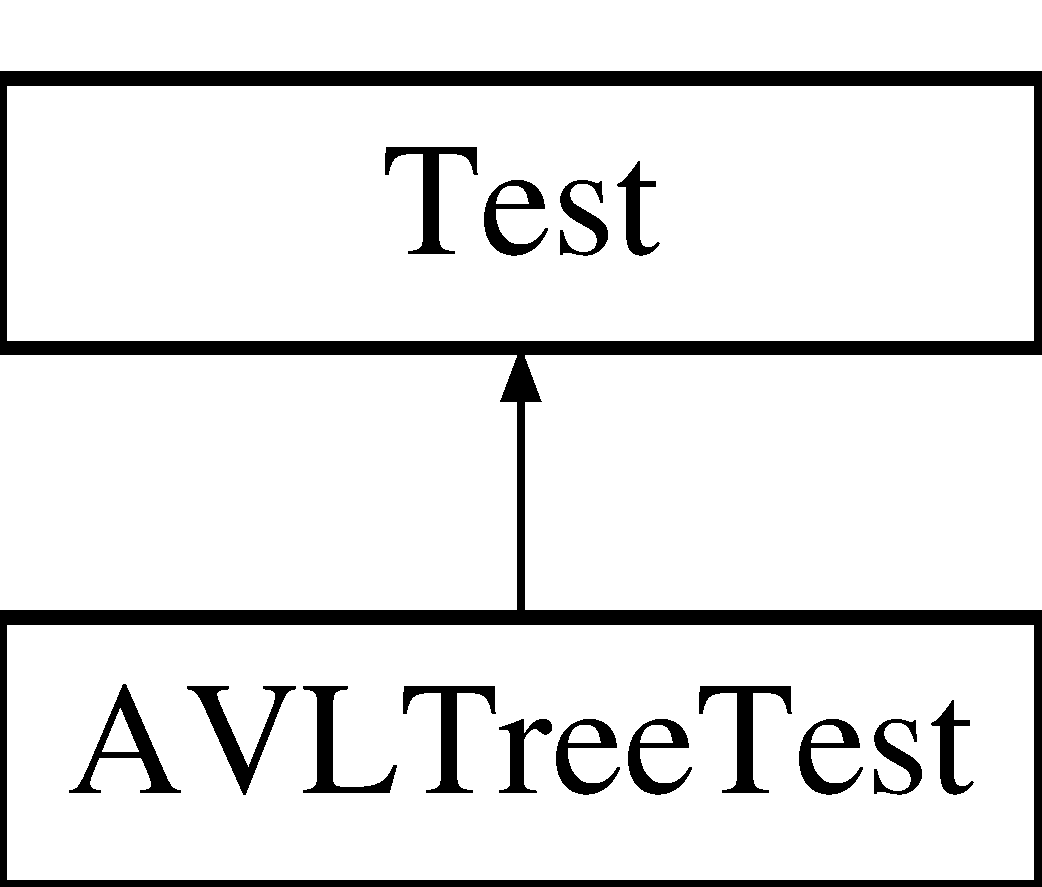
\includegraphics[height=2.000000cm]{classAVLTreeTest}
\end{center}
\end{figure}


The documentation for this class was generated from the following file\-:\begin{DoxyCompactItemize}
\item 
/home/travis/build/ob-\/algdati-\/ws17/blatt-\/7-\/aufgabe-\/1-\/create-\/a-\/new-\/team/test/test\-\_\-avl\-\_\-tree.\-h\end{DoxyCompactItemize}

\hypertarget{structavl__tree_1_1node}{\section{avl\-\_\-tree\-:\-:node Struct Reference}
\label{structavl__tree_1_1node}\index{avl\-\_\-tree\-::node@{avl\-\_\-tree\-::node}}
}


Entry of A\-V\-L-\/\-Tree.  




{\ttfamily \#include $<$avl\-\_\-tree.\-h$>$}

\subsection*{Public Member Functions}
\begin{DoxyCompactItemize}
\item 
\hyperlink{structavl__tree_1_1node_a94e7fa472a575bbcae1e506c4c8b3534}{node} (int)
\begin{DoxyCompactList}\small\item\em Creates new node. \end{DoxyCompactList}\item 
vector$<$ int $>$ $\ast$ \hyperlink{structavl__tree_1_1node_a6932b4c28a69e1adc86f41f74e16cd6e}{preorder} () const 
\begin{DoxyCompactList}\small\item\em Get subtree from this node in 'preorder'. \end{DoxyCompactList}\item 
vector$<$ int $>$ $\ast$ \hyperlink{structavl__tree_1_1node_ac0a51c1a20c50c9c4e0d7037e28afbc2}{inorder} () const 
\begin{DoxyCompactList}\small\item\em Get subtree from this node in 'inorder'. \end{DoxyCompactList}\item 
vector$<$ int $>$ $\ast$ \hyperlink{structavl__tree_1_1node_abe9f3981d8b35f0816657345eeada0a2}{postorder} () const 
\begin{DoxyCompactList}\small\item\em Get subtree from this node in 'postorder'. \end{DoxyCompactList}\end{DoxyCompactItemize}
\subsection*{Public Attributes}
\begin{DoxyCompactItemize}
\item 
\hyperlink{structavl__tree_1_1node}{node} $\ast$ \hyperlink{structavl__tree_1_1node_a3e7851f7104dd71af924b27e70d80f3a}{left} = nullptr
\item 
\hyperlink{structavl__tree_1_1node}{node} $\ast$ \hyperlink{structavl__tree_1_1node_aff21ea47ae19da99113bd7900fb69785}{right} = nullptr
\item 
int \hyperlink{structavl__tree_1_1node_a07b67fe6e79e2272835dd6485272b823}{key}
\item 
int \hyperlink{structavl__tree_1_1node_a57a93259cb3f71b15fe737a559d8f0cc}{height} = 1
\end{DoxyCompactItemize}


\subsection{Detailed Description}
Entry of A\-V\-L-\/\-Tree. 

Consists of key and pointers to its children. 

\subsection{Constructor \& Destructor Documentation}
\hypertarget{structavl__tree_1_1node_a94e7fa472a575bbcae1e506c4c8b3534}{\index{avl\-\_\-tree\-::node@{avl\-\_\-tree\-::node}!node@{node}}
\index{node@{node}!avl_tree::node@{avl\-\_\-tree\-::node}}
\subsubsection[{node}]{\setlength{\rightskip}{0pt plus 5cm}avl\-\_\-tree\-::node\-::node (
\begin{DoxyParamCaption}
\item[{int}]{key}
\end{DoxyParamCaption}
)}}\label{structavl__tree_1_1node_a94e7fa472a575bbcae1e506c4c8b3534}


Creates new node. 


\begin{DoxyParams}{Parameters}
{\em key} & Key of node \\
\hline
\end{DoxyParams}


\subsection{Member Function Documentation}
\hypertarget{structavl__tree_1_1node_ac0a51c1a20c50c9c4e0d7037e28afbc2}{\index{avl\-\_\-tree\-::node@{avl\-\_\-tree\-::node}!inorder@{inorder}}
\index{inorder@{inorder}!avl_tree::node@{avl\-\_\-tree\-::node}}
\subsubsection[{inorder}]{\setlength{\rightskip}{0pt plus 5cm}vector$<$ int $>$ $\ast$ avl\-\_\-tree\-::node\-::inorder (
\begin{DoxyParamCaption}
{}
\end{DoxyParamCaption}
) const}}\label{structavl__tree_1_1node_ac0a51c1a20c50c9c4e0d7037e28afbc2}


Get subtree from this node in 'inorder'. 

\begin{DoxyReturn}{Returns}
subtree in 'inorder' 
\end{DoxyReturn}
\hypertarget{structavl__tree_1_1node_abe9f3981d8b35f0816657345eeada0a2}{\index{avl\-\_\-tree\-::node@{avl\-\_\-tree\-::node}!postorder@{postorder}}
\index{postorder@{postorder}!avl_tree::node@{avl\-\_\-tree\-::node}}
\subsubsection[{postorder}]{\setlength{\rightskip}{0pt plus 5cm}vector$<$ int $>$ $\ast$ avl\-\_\-tree\-::node\-::postorder (
\begin{DoxyParamCaption}
{}
\end{DoxyParamCaption}
) const}}\label{structavl__tree_1_1node_abe9f3981d8b35f0816657345eeada0a2}


Get subtree from this node in 'postorder'. 

\begin{DoxyReturn}{Returns}
subtree in 'postorder' 
\end{DoxyReturn}
\hypertarget{structavl__tree_1_1node_a6932b4c28a69e1adc86f41f74e16cd6e}{\index{avl\-\_\-tree\-::node@{avl\-\_\-tree\-::node}!preorder@{preorder}}
\index{preorder@{preorder}!avl_tree::node@{avl\-\_\-tree\-::node}}
\subsubsection[{preorder}]{\setlength{\rightskip}{0pt plus 5cm}vector$<$ int $>$ $\ast$ avl\-\_\-tree\-::node\-::preorder (
\begin{DoxyParamCaption}
{}
\end{DoxyParamCaption}
) const}}\label{structavl__tree_1_1node_a6932b4c28a69e1adc86f41f74e16cd6e}


Get subtree from this node in 'preorder'. 

\begin{DoxyReturn}{Returns}
subtree in 'preorder' 
\end{DoxyReturn}


\subsection{Member Data Documentation}
\hypertarget{structavl__tree_1_1node_a57a93259cb3f71b15fe737a559d8f0cc}{\index{avl\-\_\-tree\-::node@{avl\-\_\-tree\-::node}!height@{height}}
\index{height@{height}!avl_tree::node@{avl\-\_\-tree\-::node}}
\subsubsection[{height}]{\setlength{\rightskip}{0pt plus 5cm}int avl\-\_\-tree\-::node\-::height = 1}}\label{structavl__tree_1_1node_a57a93259cb3f71b15fe737a559d8f0cc}
Current height of this node. \hypertarget{structavl__tree_1_1node_a07b67fe6e79e2272835dd6485272b823}{\index{avl\-\_\-tree\-::node@{avl\-\_\-tree\-::node}!key@{key}}
\index{key@{key}!avl_tree::node@{avl\-\_\-tree\-::node}}
\subsubsection[{key}]{\setlength{\rightskip}{0pt plus 5cm}int avl\-\_\-tree\-::node\-::key}}\label{structavl__tree_1_1node_a07b67fe6e79e2272835dd6485272b823}
Key identifying this node. \hypertarget{structavl__tree_1_1node_a3e7851f7104dd71af924b27e70d80f3a}{\index{avl\-\_\-tree\-::node@{avl\-\_\-tree\-::node}!left@{left}}
\index{left@{left}!avl_tree::node@{avl\-\_\-tree\-::node}}
\subsubsection[{left}]{\setlength{\rightskip}{0pt plus 5cm}{\bf node}$\ast$ avl\-\_\-tree\-::node\-::left = nullptr}}\label{structavl__tree_1_1node_a3e7851f7104dd71af924b27e70d80f3a}
Left child of this node. \hypertarget{structavl__tree_1_1node_aff21ea47ae19da99113bd7900fb69785}{\index{avl\-\_\-tree\-::node@{avl\-\_\-tree\-::node}!right@{right}}
\index{right@{right}!avl_tree::node@{avl\-\_\-tree\-::node}}
\subsubsection[{right}]{\setlength{\rightskip}{0pt plus 5cm}{\bf node}$\ast$ avl\-\_\-tree\-::node\-::right = nullptr}}\label{structavl__tree_1_1node_aff21ea47ae19da99113bd7900fb69785}
Right child of this node. 

The documentation for this struct was generated from the following files\-:\begin{DoxyCompactItemize}
\item 
/home/travis/build/ob-\/algdati-\/ws17/blatt-\/7-\/aufgabe-\/1-\/create-\/a-\/new-\/team/avl\-\_\-tree/avl\-\_\-tree.\-h\item 
/home/travis/build/ob-\/algdati-\/ws17/blatt-\/7-\/aufgabe-\/1-\/create-\/a-\/new-\/team/avl\-\_\-tree/avl\-\_\-tree.\-cpp\end{DoxyCompactItemize}

%--- End generated contents ---

% Index
\newpage
\phantomsection
\addcontentsline{toc}{chapter}{Index}
\printindex

\end{document}
